\documentclass[tikz,border=8pt]{standalone}
\usepackage{amsmath}
\usetikzlibrary{arrows.meta,positioning}

\begin{document}
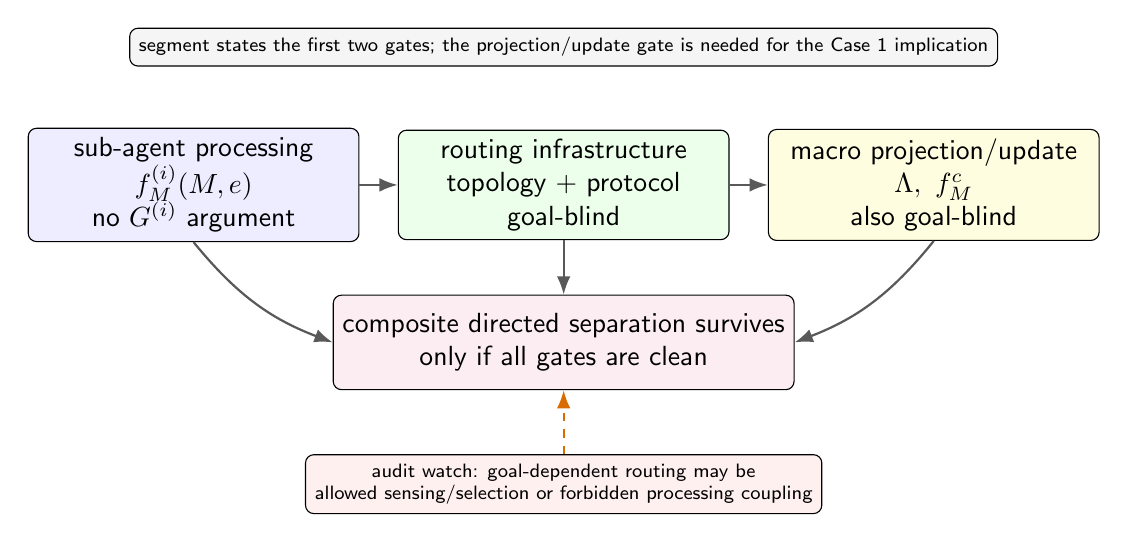
\begin{tikzpicture}[
  font=\sffamily,
  gate/.style={draw, rounded corners=3pt, align=center, minimum width=42mm, minimum height=12mm, fill=white},
  note/.style={draw, rounded corners=3pt, align=center, font=\sffamily\scriptsize, fill=white},
  arrow/.style={-Latex, thick, draw=black!65},
  warn/.style={-Latex, thick, dashed, draw=orange!85!black}
]

\node[gate, fill=blue!7] (sub) at (-4.7,1.25)
  {sub-agent processing\\$f_M^{(i)}(M,e)$\\no $G^{(i)}$ argument};
\node[gate, fill=green!8] (route) at (0,1.25)
  {routing infrastructure\\topology + protocol\\goal-blind};
\node[gate, fill=yellow!12] (proj) at (4.7,1.25)
  {macro projection/update\\$\Lambda,\ f_M^c$\\also goal-blind};

\draw[arrow] (sub.east) -- (route.west);
\draw[arrow] (route.east) -- (proj.west);

\node[gate, fill=purple!7, minimum width=48mm] (survive) at (0,-0.75)
  {composite directed separation survives\\only if all gates are clean};
\draw[arrow] (sub.south) to[bend right=15] (survive.west);
\draw[arrow] (route.south) -- (survive.north);
\draw[arrow] (proj.south) to[bend left=15] (survive.east);

\node[note, fill=red!6, minimum width=61mm] (case2) at (0,-2.55)
  {audit watch: goal-dependent routing may be\\allowed sensing/selection or forbidden processing coupling};
\draw[warn] (case2.north) -- (survive.south);

\node[note, fill=gray!8, minimum width=78mm] at (0,3.0)
  {segment states the first two gates; the projection/update gate is needed for the Case 1 implication};

\end{tikzpicture}
\end{document}
